% !TEX root = morphkasten.tex

\section{Mini-Computer}


%##############
\subsection{Raspberry Pi 1}

\begin{figure}[h!]%Position festigen
\centering
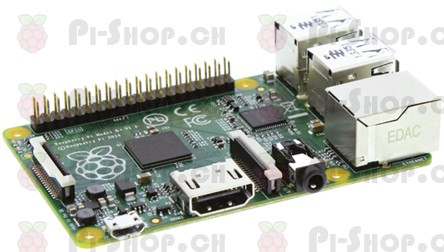
\includegraphics[width=0.5\textwidth]{fig/PI1.jpg}
\caption{Raspberry Pi 1 (Quelle: https://www.pi-shop.ch)}
\label{fig:PI1}
\end{figure}

\begin{table}[h]
\begin{tabular}{p{0.5\textwidth} | p{0.5\textwidth}}


 \textbf{Vorteile} & \textbf{Nachteile} \\ \hline
	 
\begin{itemize}
\item Zuverlässig
\item Einfache Ansteuerung
\item Kompatible Komponenten (Kamera)
\item Geläufiges Betriebssystem
\item Geringer Energieverbrauch
\end{itemize}

 
 &
 
\begin{itemize}
\item Wenig Leistung (Echtzeit)
\item Platzverbrauch auf Fahrzeug
\end{itemize}

\end{tabular}
\end{table}

\begin{table}[h]
\begin{tabular}{p{0.5\textwidth}p{0.5\textwidth}}


 \textbf{Risiken} & \\ \hline
	 
\begin{itemize}
\item Echtzeitbildverarbeitung funktioniert nicht
\item Benötigt zu viel Platz auf Fahrzeug
\end{itemize}

 
\end{tabular}
\end{table}

\pagebreak


%##############
\subsection{Raspberry Pi 2}

\begin{figure}[h!]%Position festigen
\centering
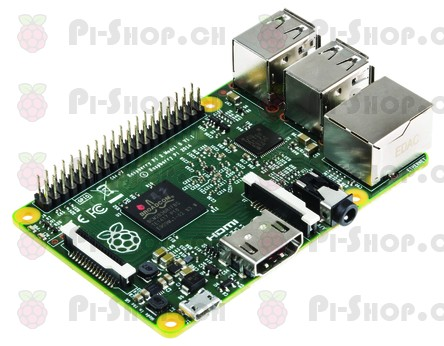
\includegraphics[width=0.5\textwidth]{fig/PI2.jpg}
\caption{Raspberry Pi 2 (Quelle: https://www.pi-shop.ch)}
\label{fig:PI2}
\end{figure}

\begin{table}[h]
\begin{tabular}{p{0.5\textwidth} | p{0.5\textwidth}}


 \textbf{Vorteile} & \textbf{Nachteile} \\ \hline
	 
\begin{itemize}
\item Hohe Leistung (Echtzeit)
\item Zuverlässig
\item Einfache Ansteuerung
\item Kompatible Komponenten (Kamera)
\item Geläufiges Betriebssystem
\item Geringer Energieverbrauch
\end{itemize}

 
 &
 
\begin{itemize}
\item Energieverbrauch zu hoch
\item Platzverbrauch auf Fahrzeug
\end{itemize}

\end{tabular}
\end{table}

\begin{table}[h]
\begin{tabular}{p{0.5\textwidth}p{0.5\textwidth}}


 \textbf{Risiken} & \\ \hline
	 
\begin{itemize}
\item Verbraucht zu viel Energie
\item Echtzeitbildverarbeitung funktioniert trotzdem nicht
\item Benötigt zu viel Platz auf Fahrzeug
\end{itemize}


 
\end{tabular}
\end{table}

\pagebreak

%##############
\subsection{Banana Pi}

\begin{figure}[h!]%Position festigen
\centering
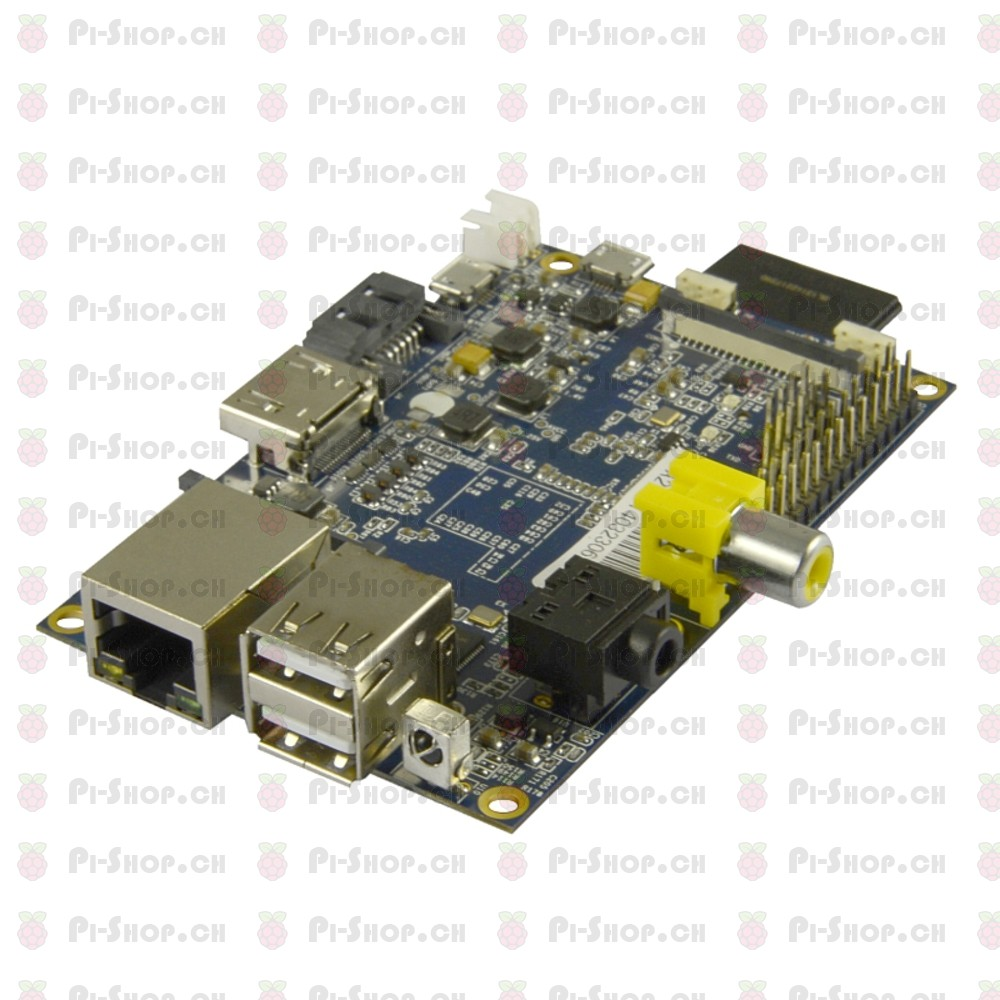
\includegraphics[width=0.5\textwidth]{fig/PIBanana.jpg}
\caption{Banana Pi (Quelle: https://www.pi-shop.ch)}
\label{fig:Banana Pi}
\end{figure}

\begin{table}[h]
\begin{tabular}{p{0.5\textwidth} | p{0.5\textwidth}}


 \textbf{Vorteile} & \textbf{Nachteile} \\ \hline
	 
\begin{itemize}
\item Minimal günstiger
\item Geläufiges Betriebssystem
\item Geringer Energieverbrauch
\end{itemize}

 
 &
 
\begin{itemize}
\item Keinerlei Erfahrung
\item Wenig Leistung (Echtzeit)
\item Platzverbrauch auf Fahrzeug
\end{itemize}

\end{tabular}
\end{table}

\begin{table}[h]
\begin{tabular}{p{0.5\textwidth}p{0.5\textwidth}}


 \textbf{Risiken} & \\ \hline
	 
\begin{itemize}
\item Zu wenig Zeit zum Einarbeiten
\item Echtzeitbildverarbeitung funktioniert nicht
\item Benötigt zu viel Platz auf Fahrzeug
\end{itemize}

 
\end{tabular}
\end{table}

\pagebreak